% {{{ Preamble ----------------------------------------------------------------
\documentclass{beamer}

% encodings, fonts etc.
\usepackage[utf8x]{inputenc}
\usepackage[T1]{fontenc}

% Hold kæft utf
\makeatletter
\def\UTFviii@defined#1{%
  \ifx#1\relax
      ?%
  \else\expandafter
    #1%
  \fi
}

\makeatother

% math packages
\usepackage{amsmath, amssymb, amsthm}
\usepackage{mathtools}

% beamer configuration
\usetheme{Copenhagen}
%\useoutertheme{infolines}
%\usetheme{metropolis}
\beamertemplatenavigationsymbolsempty
%\setbeamertemplate{theorems}[numbered]
\setbeamersize{description width=2.0em}

%\usepackage{pgfpages}
%\setbeameroption{show notes}
%\setbeameroption{show notes on second screen=right}

% algorithms
\usepackage{algorithm}
\usepackage[noend]{algpseudocode}

% misc. packages
\usepackage{float}
\usepackage{varwidth}
\usepackage{listings}
\lstset{
  %breaklines=true,
  keepspaces=true,
  %frame=ltrb,
  %framesep=1pt,
  %commentstyle=\color{grey},
  basicstyle=\ttfamily\tiny,
  %numbers=left,
  title=\lstname,
  %columns=fullflexible,
  inputencoding=utf8,
  extendedchars=true,
}

% graphics and tikz
\usepackage{pgf}
\usepackage{tikz}
\usetikzlibrary{positioning,arrows,calc}
\tikzset{
    on grid,
    node distance=3cm,
    auto,
    block/.style = {
        draw,
        shape=rectangle,
        minimum height=3em,
        minimum width=3em,
        line width=1pt
    },
    control/.style = {
        draw,
        shape=circle,
        minimum height=7em,
        minimum width=3em,
        line width=1pt
    },
    mux/.style = {
        draw,
        shape=rectangle,
        minimum height=1.5em,
        minimum width=1em,
        line width=1pt
    },
    empty/.style = {
        shape=rectangle,
        minimum height=3em,
        minimum width=3em
    },
    >=latex',
}


% mathematics
\newtheorem{proposition}{Proposition}

\renewcommand{\tt}{\texttt}

% title page
\title{Single Cycle MIPS Processor}
\author[Carl-Johannes Johnsen]{
  \mbox{Carl-Johannes Johnsen}}
\institute{Department of Computer Science\\
           University of Copenhagen}
%\date{December 22, 2016}
% }}} -------------------------------------------------------------------------

\begin{document}

% {{{ Title page --------------------------------------------------------------
\frame{\titlepage}
% }}} -------------------------------------------------------------------------

% {{{ Table of contents -------------------------------------------------------
%\begin{frame}
%  \frametitle{Outline}
%  \tableofcontents
%\end{frame}
% }}} -------------------------------------------------------------------------
\section{Introduction}
\begin{frame}
    In this lecture, we will be combining the core components into a single
    cycle MIPS processor.

    \vspace{\baselineskip}
    Then we will be looking at writing our first program, in order to verify
    that the processor works as intended.

    \vspace{\baselineskip}
    Then we will be extending the processor, so that it can handle more
    instructions. Following each added instruction, we will be extending our
    initial program with the newly added instructions.

    \vspace{\baselineskip}
    Finally, we will be writing two larger programs, and look into compiling
    them into hex values, that the processor can read.
\end{frame}
\section{Wiring up the processor}
\begin{frame}
    Now that we have all the components and their busses, wiring up the
    processor is straightforward. We just need to declare the bus names, so
    that each process gets the bus with the corresponding name, and then SME
    will handle the wiring for us.

    \vspace{\baselineskip}
    Note: as previously mentioned, the PC register and the Write Buffer should
    be clocked processes.
\end{frame}
\begin{frame}
    \begin{figure}
        \centering
        \scalebox{0.5}{
            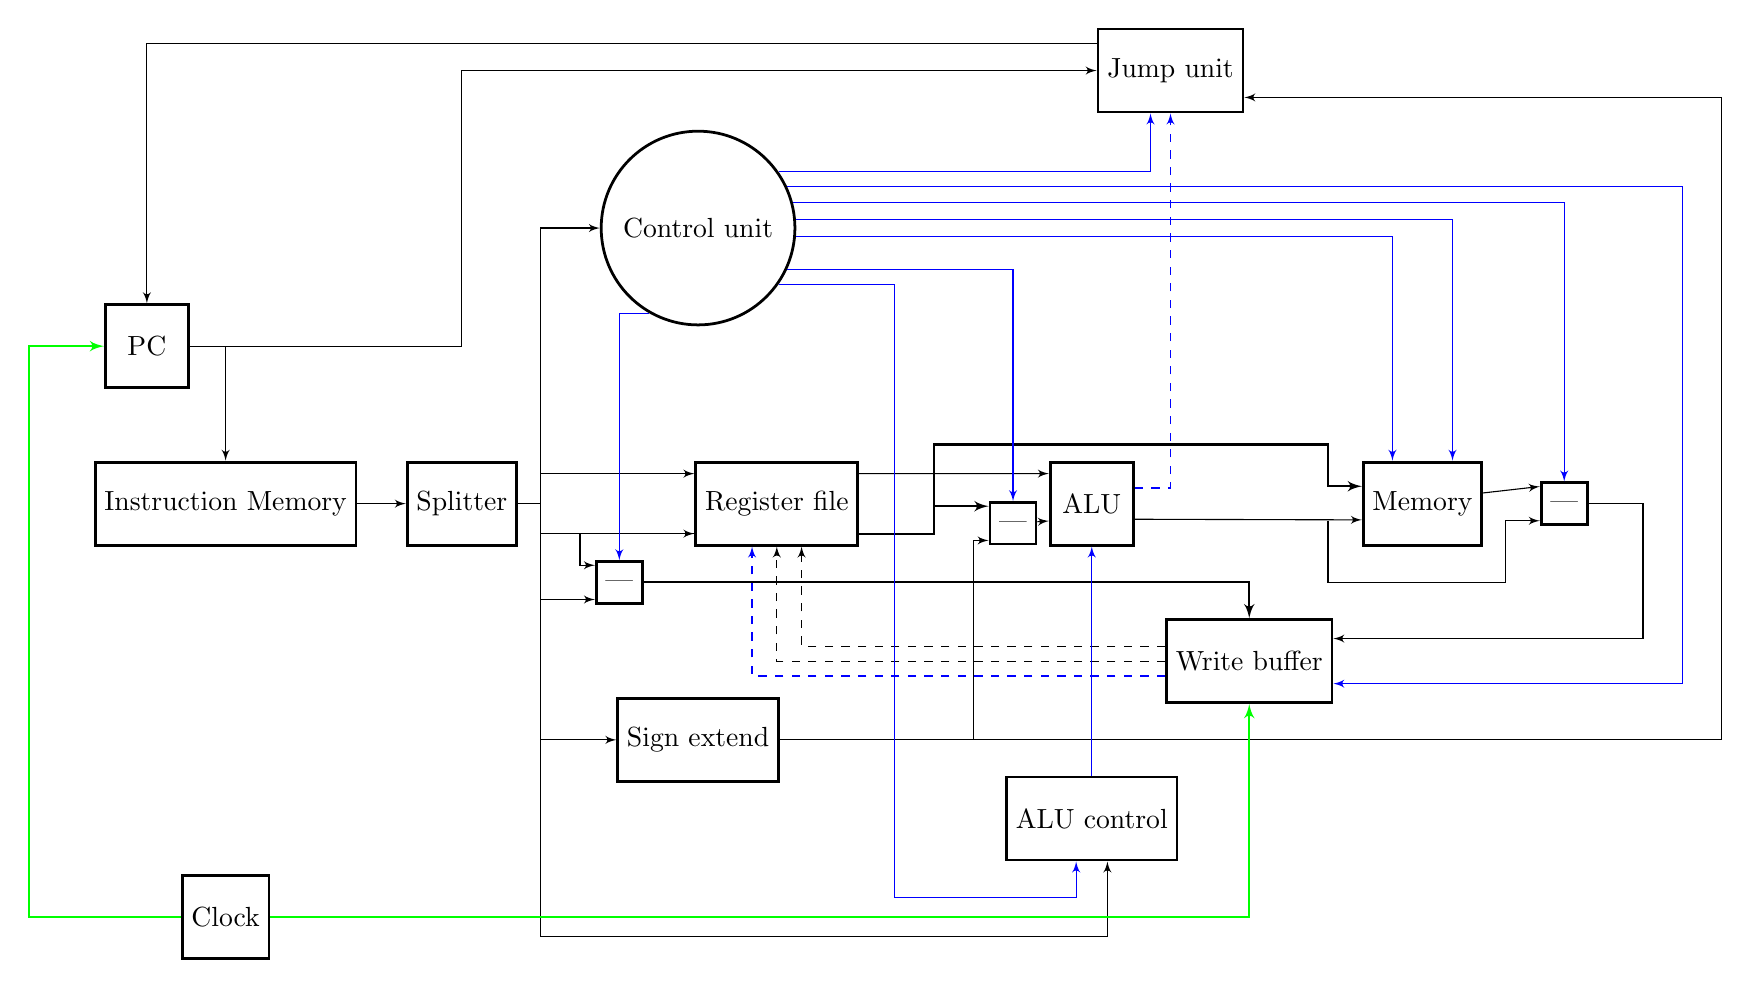
\begin{tikzpicture}
                \node[block] (reg) at (0,0) {Register file};
                \node[control] (cont) at (-1,3.5) {Control unit};
                \node[block] (jump) at (5,5.5) {Jump unit};
                \node[empty] (splitspace) at (-3,0) {};
                \node[block] (split) at (-4,0) {Splitter};
                \node[block] (if) at (-7,0) {Instruction Memory};
                \node[block] (sign) at (-1,-3) {Sign extend};
                \node[block] (alu) at (4,0) {ALU};
                \node[block] (alucont) at (4,-4) {ALU control};
                \node[block] (mem) at (8.2,0) {Memory};
                \node[mux] (memread) at (10,0) {|};
                \node[mux] (imm) at (3, -0.25) {|};
                \node[mux] (regdst) at (-2,-1) {|};
                \node[block] (pc) at (-8, 2) {PC};
                \node[block] (writebuf) at (6, -2) {Write buffer};

                \path[draw, ->] (if) -- (split);
                \path[draw, -] (split) -- (splitspace.center);
                \path[draw, ->] (splitspace.center) |- (sign);
                \path[draw, ->] (splitspace.center) |- (cont);
                \path[draw, ->] (splitspace.center) |- (reg.160);
                \path[draw, ->] (splitspace.center) |- (reg.200);
                %\path[draw, ->] (splitspace.center) |- (alucont.200);
                \path[draw, ->] (splitspace.center) |- (2,-5.5) -| (alucont.290);
                \path[draw, ->] (splitspace.center) |- (regdst.215);
                \path[draw, ->] (reg.200) -| (-2.5, -0.5) |- (regdst.145);
                %\path[draw, ->] (alucont) -| (12.5, 0) |- (jump);
                \path[draw, thick, ->] (reg.340) -| (2,-0.25) |- (imm.145);
                \path[draw, thick, ->] (2,-0.25) |- (3,0.75) -- (7,0.75) |-
                (mem.164);
                \path[draw, ->] (reg.20) -- (alu.145);
                \path[draw, ->, dashed, color=blue] (alu.20) -| (jump);
                %\path[draw, ->] (alu.340) -- (jal);
                %\path[draw, ->] (jal) -- (mem.196);
                %\path[draw, ->] (jal) -- (writebuf);
                \path[draw, ->] (alu.340) -- (mem.195);
                \path[draw, ->] (imm) -- (alu.202);
                \path[draw, ->] (7, -0.22) |- (8, -1) -| (9.25,-0.5) |-
                (memread.215);
                \path[draw, ->] (mem.10) -- (memread.145);
                \path[draw, ->] (sign) -| (2.5, -1) |- (imm.215);
                \path[draw, ->] (2.5,-3) -| (12, 0) |- (jump.340);
                %\path[draw, thick, ->] (regdst) -| (5, -0.6) |- (jal.210);
                \path[draw, thick, ->] (regdst) -| (writebuf);
                \path[draw, ->] (pc) -| (if);
                \path[draw, ->] (pc) -| (-4, 4) |- (jump);
                \path[draw, ->] (jump.160) -| (pc);
                \path[draw, ->] (memread) -| (11, -1) |- (writebuf.15);
                \path[draw, dashed, ->] (writebuf.170) -| (reg.300);
                \path[draw, dashed, ->] (writebuf) -| (reg);
                \path[draw, dashed, ->, color=blue] (writebuf.190) -| (reg.240);

                \path[draw, ->, color=blue] (alucont) -- (alu);
                \path[draw, ->, color=blue] (cont.35) -| (jump.245);
                \path[draw, ->, color=blue] (cont.25) -| (11.5,0) |-
                (writebuf.345);
                \path[draw, ->, color=blue] (cont.15) -| (memread);
                \path[draw, ->, color=blue] (cont.5) -| (mem.55);
                \path[draw, ->, color=blue] (cont.355) -| (mem.125);
                \path[draw, ->, color=blue] (cont.335) -| (imm);
                \path[draw, ->, color=blue] (cont.325) -| (1.5, -4) |-
                (2, -5) -| (alucont.250);
                \path[draw, ->, color=blue] (cont.240) -| (regdst);

                \node[block] (clock) at (-7, -5.25) {Clock};
                \path[draw, ->, thick, color=green] (clock) -| (-9.5,0) |- (pc);
                \path[draw, ->, thick, color=green] (clock) -| (writebuf);
            \end{tikzpicture}
        }
\end{figure}
\end{frame}
\section{Writing the first program}
\begin{frame}
    As mentioned before, the first single cycle MIPS processor should be able
    to handle \texttt{add}, \texttt{sub}, \texttt{and}, \texttt{or},
    \texttt{slt}, \texttt{sw}, \texttt{lw} and \texttt{beq}. As such, the first
    program should consist of these.
\end{frame}
\begin{frame}
    \begin{center}
        \scalebox{0.7}{
            \begin{tabular}{rllllllll}
                \hline
                Address & Instruction & opcode & rs & rt & rd/imm & shmt & funct & hex \\
                \hline
                \texttt{0x00} & \texttt{add \$3 \$1 \$2} & \texttt{0x00} &
                \texttt{0x01} & \texttt{0x02} & \texttt{0x03} & \texttt{0x00} &
                \texttt{0x20} & \texttt{0x00221820} \\ % 5 + 2 = 7

                \texttt{0x04} & \texttt{sub \$4 \$3 \$2} & \texttt{0x00} &
                \texttt{0x03} & \texttt{0x02} & \texttt{0x04} & \texttt{0x00} &
                \texttt{0x22} & \texttt{0x00622022} \\ %  7 - 2 = 5

                \texttt{0x08} & \texttt{and \$5 \$3 \$1} & \texttt{0x00} &
                \texttt{0x03} & \texttt{0x03} & \texttt{0x05} & \texttt{0x00} &
                \texttt{0x24} & \texttt{0x00612824} \\ % 7 and 5 = 5

                \texttt{0x0C} & \texttt{and \$6 \$3 \$1} & \texttt{0x00} &
                \texttt{0x03} & \texttt{0x03} & \texttt{0x06} & \texttt{0x00} &
                \texttt{0x25} & \texttt{0x00613025} \\ % 7 or 5 = 7

                \texttt{0x10} & \texttt{slt \$7 \$6 \$5} & \texttt{0x00} &
                \texttt{0x06} & \texttt{0x05} & \texttt{0x07} & \texttt{0x00} &
                \texttt{0x2A} & \texttt{0x00C5382A} \\ % 7 < 5 = 1

                \texttt{0x14} & \texttt{sw \$6  0x0(\$0)} & \texttt{0x2B} &
                \texttt{0x00} & \texttt{0x06} & \texttt{0x0000} & - &
                - & \texttt{0xAC060000} \\ % M[0] = 7

                \texttt{0x18} & \texttt{lw \$8  0x0(\$0)} & \texttt{0x23} &
                \texttt{0x00} & \texttt{0x07} & \texttt{0x0000} & - &
                - & \texttt{0x8C070000} \\ % $8 = M[0] (= 7)

                \texttt{0x1C} & \texttt{beq \$5 \$4 0x4} & \texttt{0x04} &
                \texttt{0x05} & \texttt{0x04} & \texttt{0x0004} & - &
                - & \texttt{0x10A40004} \\ % if 5 == 5 then skip next

                \texttt{0x20} & \texttt{add \$9 \$8 \$6} & \texttt{0x00} &
                \texttt{0x08} & \texttt{0x06} & \texttt{0x09} & \texttt{0x00} &
                \texttt{0x20} & \texttt{0x01064820} \\ % 7 + 7 = 14 // should not run!

                \texttt{0x24} & \texttt{add \$10 \$8 \$6} & \texttt{0x00} &
                \texttt{0x08} & \texttt{0x06} & \texttt{0x0A} & \texttt{0x00} &
                \texttt{0x20} & \texttt{0x01065020} \\ % 7 + 7 = 14
                \hline
            \end{tabular}
        }
    \end{center}
\end{frame}
\begin{frame}
    Inserting this program into the Instruction Memory is straightforward: just
    create an \texttt{byte} array, which is initialized to the hex values from
    the instruction column in the previous table.

    \vspace{\baselineskip}
    Since we do not have any way of feeding values into the Register File at
    this moment, we are going to hardcode registers 1 and 2 with the values 5
    and 2 respectively.
\end{frame}
\begin{frame}
    When the program has finished, the contents of the register file should be
    as this table:
    \begin{table}
        \centering
        \begin{tabular}{rrrrrrrrrrrrrrrrrrrr}
            \hline
            Address & 0 & 1 & 2 & 3 & 4 & 5 & 6 & 7 & 8 & 9 & 10 \\
            \hline
            Value & 0 & 5 & 2 & 7 & 5 & 5 & 7 & 1 & 7 & 0 & 14 \\
            \hline
        \end{tabular}
    \end{table}
\end{frame}

\section{Extending the accepted instruction set}
\subsection{Additional simple R format instructions}
\begin{frame}
    We start by implementing the simple remaining R format instructions:
    \begin{itemize}
        \item \texttt{addu}
        \item \texttt{subu}
        \item \texttt{xor}
        \item \texttt{nor}
        \item \texttt{sltu}
    \end{itemize}
    The only modification that we need to do, is to extend the ALUOperation
    \texttt{enum}, and then add the remaining \texttt{case}s in the ALU Control
    and in the ALU.
\end{frame}

\subsection{Immediate instructions}
\begin{frame}
    The next instruction we want to add is the \texttt{ori} instruction, as we
    can then feed initial values into the Register File, and thus remove the
    hardcoding in the Register File. As we are extending the processor to
    handle the \texttt{ori} instruction, we should also add support for these
    instructions, as it requires the same amount of work:
    \begin{itemize}
        \item \texttt{addi}
        \item \texttt{addiu}
        \item \texttt{slti}
        \item \texttt{sltiu}
        \item \texttt{andi}
        \item \texttt{xori}
    \end{itemize}
\end{frame}
\begin{frame}
    For the logical immediates, we need to ensure that the Sign Extend does not
    sign extend, but rather zero extends. To do this, we add an additional
    control signal in the Control Unit: \texttt{LogicalImmediate}. If this flag
    is set to \texttt{1}, the sign extend should not sign extend.

    \vspace{\baselineskip}
    Then we just need to extend the opcode and the ALUOp \texttt{enum}, and add
    the remaining \texttt{case}s in the Control Unit and the ALU Control.
\end{frame}

\subsection{Jump instruction}
\begin{frame}
    We are going to introduce another format: the J format. This format is used
    for executing the \texttt{j} instruction.

    \vspace{\baselineskip}
    The first step is to extend the Splitter, as it should send the lower 26
    bits to the Jump Unit.

    \vspace{\baselineskip}
    Then the opcode \texttt{enum} should be extended, and the \texttt{case} for
    \texttt{j} should be added to the Control Unit. The Control Unit should
    have an additional control signal: \texttt{jump}, which should go to the
    Jump Unit.
\end{frame}
\begin{frame}
    Finally, the Jump Unit should be extended to handle the \texttt{j}
    instruction.

    \vspace{\baselineskip}
    It should start by taking the 26 bits from the Splitter, and left shift by
    2, just as we did with branching. Then it should take the 4 most
    significant bits of the incremented PC, and prepend them to the shifted
    address. Finally, we add a multiplexor, which takes the computed jump
    address, the previous output address and the \texttt{jump} signal as
    inputs. If the control signal is \texttt{0}, then the original output
    should be put on the output bus, and the jump address otherwise.
\end{frame}

\subsection{Remaining branching instructions}
\begin{frame}
    Then we are going to add the remaining branching instructions:
    \begin{itemize}
        \item \texttt{bne}
        \item \texttt{blez}
        \item \texttt{bgtz}
    \end{itemize}
\end{frame}
\begin{frame}
    To implement the \texttt{bne} instruction, we are going to add another
    signal from the Control Unit to the Jump Unit: \texttt{bne}. Then we should
    split the Zero signal into two, and add a \texttt{NOT} gate, where one of
    the Zero signals should go to. Then we add a multiplexor, which takes Zero,
    not Zero and the \texttt{bne} signal as input. If the \texttt{bne} signal
    is \texttt{0}, then the output should be the original Zero, and the not
    Zero otherwise. This output should go into the \texttt{AND} gate, where the
    Zero signal was before.
\end{frame}

\subsection{Remaining jump instructions}
\begin{frame}
    Then we are going to add the remaining jump instructions:
    \begin{itemize}
        \item \texttt{jr}
        \item \texttt{jal}
        \item \texttt{jalr}
    \end{itemize}
    As these are useful when writing the larger programs later.
\end{frame}
\begin{frame}
    We start with \texttt{jr}. The instruction is in R format, so we do not
    know it is \texttt{jr}, until it has reached the ALU Control. As such, we
    are going to need a control signal from the ALU Control to the Jump Unit.
    We are also going to forward Output A from the Register File to the Jump
    Unit, as this is the address that the processor should jump to in the
    \texttt{jr} instruction.

    \vspace{\baselineskip}
    The Jump Unit should not compute the new address in the same manner as with
    the \texttt{j} instruction. This is due to the registers being a full 32
    bit, and thus can contain the whole address space.

    \vspace{\baselineskip}
    The Jump Unit should also have a multiplexor, controlling whether the jump
    address should be the immediate value, or if it should be the value from
    the instruction.
\end{frame}
\begin{frame}
    For the \texttt{jal} instruction, we are going to need an extra unit
    following the ALU.

    \vspace{\baselineskip}
    In the case of a \texttt{jal} instruction, we should store the PC+4 address
    in register \texttt{31} (which is called the \texttt{\$ra} register).
    There should be an additional control signal from the Control Unit: the
    \texttt{jal} signal. The new JAL Unit should take three inputs: the ALU
    Result, the PC+4 and the \texttt{jal} control signal. It should produce two
    outputs: the Write Address for the Write Buffer, and the value to store. If
    the \texttt{jal} signal is \texttt{1}, the JAL Unit should output the PC+4
    on the value bus, and \texttt{31} on the address bus.  Otherwise it should
    output the regular ALU Result, and the regular Write Address.
\end{frame}

\subsection{Shift instructions}
\begin{frame}
    Then we are going to add the shift instructions:
    \begin{itemize}
        \item \texttt{sll}
        \item \texttt{slr}
        \item \texttt{sra}
        \item \texttt{sllv}
        \item \texttt{srlv}
        \item \texttt{srav}
    \end{itemize}
\end{frame}
\begin{frame}
    The shifting itself is performed in the ALU, and modifying the ALU to
    handle these is straightforward.

    \vspace{\baselineskip}
    The problem is that in an R format instruction, which the shift operations
    are, the shift amount (\texttt{shamt}) is stored in its own field within
    the instruction. As such, the splitter should extract these 5 bits, and
    send them to a new multiplexor, which also takes Output A from the Register
    File.

    \vspace{\baselineskip}
    As with the \texttt{jr} instruction, we do not know it is a shifting
    instruction until it reaches the ALU Control. So to control the new
    multiplexor, we need a Control signal from the ALU Control, indicating
    whether the multiplexor should output either the \texttt{shamt} or Output A
    from the Register File.
\end{frame}

\subsection{Multiplication and Division instructions}
\begin{frame}
    Then we are going to add the multiplication and division instructions:
    \begin{itemize}
        \item \texttt{mult}
        \item \texttt{multu}
        \item \texttt{div}
        \item \texttt{divu}
    \end{itemize}
    All of these instructions put their result in two special registers: HI and
    LO. As such, to get the results from them, we are also going to need the
    following instructions:
    \begin{itemize}
        \item \texttt{mfhi}
        \item \texttt{mthi}
        \item \texttt{mflo}
        \item \texttt{mtlo}
    \end{itemize}
\end{frame}
\begin{frame}
    We start by adding the special registers. Since they are performed in the
    ALU, we might as well put them there. Then, when we are doing the
    computation, we should just put the values there, and since the
    instructions do not write to registers, touch memory or change the PC
    register, it does not matter what is put on the ALU Result or Zero busses.

    \vspace{\baselineskip}
    The instructions handling the moving to and from the HI and LO registers
    are simple to implement: just either input or output the corresponding
    register, to or from the ALU.
\end{frame}

\section{The fully extended Single Cycle MIPS processor}
\begin{frame}
    \begin{figure}
        \centering
        \scalebox{0.5}{
            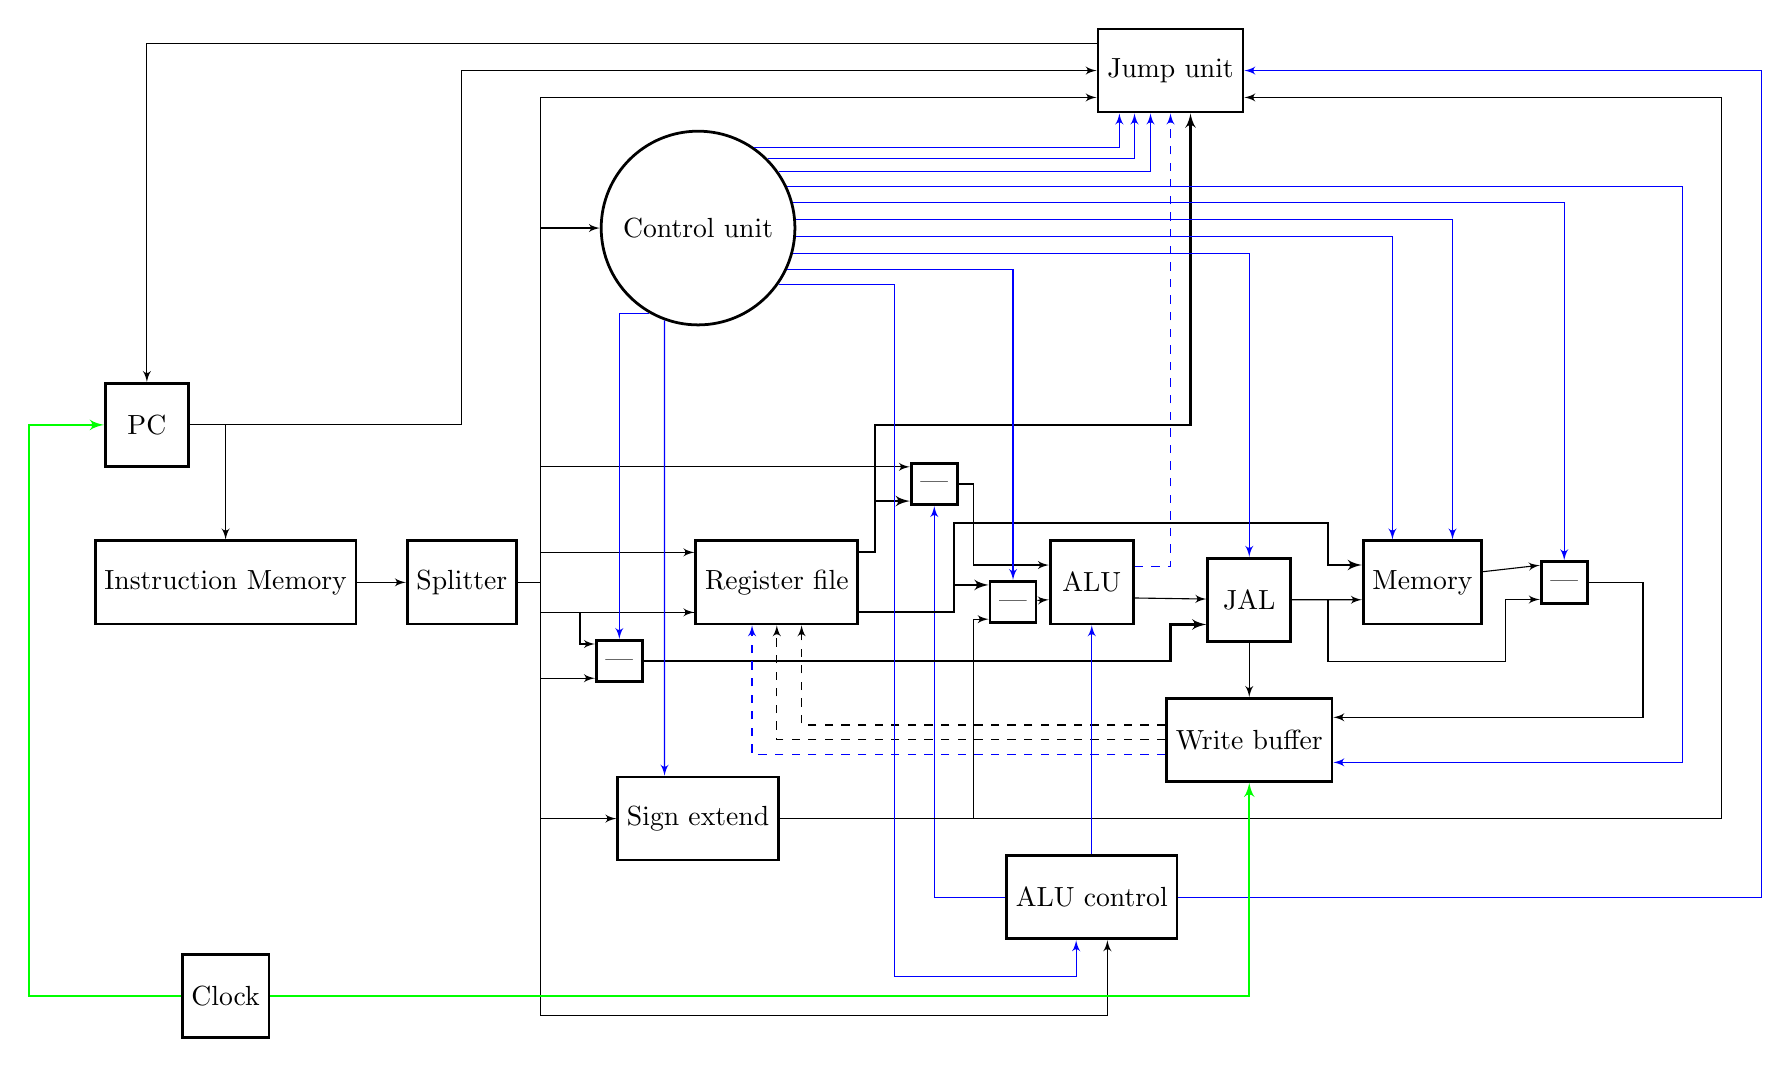
\begin{tikzpicture}
                \node[block] (reg) at (0,0) {Register file};
                \node[control] (cont) at (-1,4.5) {Control unit};
                \node[block] (jump) at (5,6.5) {Jump unit};
                \node[empty] (splitspace) at (-3,0) {};
                \node[block] (split) at (-4,0) {Splitter};
                \node[block] (if) at (-7,0) {Instruction Memory};
                \node[block] (sign) at (-1,-3) {Sign extend};
                \node[block] (alu) at (4,0) {ALU};
                \node[block] (alucont) at (4,-4) {ALU control};
                \node[block] (mem) at (8.2,0) {Memory};
                \node[block] (jal) at (6,-0.22) {JAL};
                \node[mux] (memread) at (10,0) {|};
                \node[mux] (shmt) at (2,1.25) {|};
                \node[mux] (imm) at (3, -0.25) {|};
                \node[mux] (regdst) at (-2,-1) {|};
                \node[block] (pc) at (-8, 2) {PC};
                \node[block] (writebuf) at (6, -2) {Write buffer};

                \path[draw, ->] (if) -- (split);
                \path[draw, -] (split) -- (splitspace.center);
                \path[draw, ->] (splitspace.center) |- (sign);
                \path[draw, ->] (splitspace.center) |- (cont);
                \path[draw, ->] (splitspace.center) |- (reg.160);
                \path[draw, ->] (splitspace.center) |- (reg.200);
                \path[draw, ->] (splitspace.center) |- (jump.200);
                \path[draw, ->] (splitspace.center) |- (2,-5.5) -| (alucont.290);
                \path[draw, ->] (splitspace.center) |- (regdst.215);
                \path[draw, ->] (splitspace.center) |- (shmt.145);
                \path[draw, ->] (reg.200) -| (-2.5, -0.5) |- (regdst.145);
                \path[draw, ->, color=blue] (alucont) -| (12.5, 0) |- (jump);
                \path[draw, ->, color=blue] (alucont) -| (shmt);
                \path[draw, thick, ->] (reg.340) -| (2.25,-0.25) |- (imm.145);
                \path[draw, thick, ->] (2.25,-0.25) |- (3,0.75) -- (7,0.75) |-
                (mem.164);
                \path[draw, thick, ->] (reg.20) -| (1.25,0.5) |- (shmt.215);
                \path[draw, thick, -] (1.25,0.5) |- (4,2);
                \path[draw, thick, ->] (4,2) -| (jump.295);
                \path[draw, ->] (shmt) -| (2.5, 0.5) |- (alu.158);
                \path[draw, ->, dashed, color=blue] (alu.20) -| (jump);
                \path[draw, ->] (alu.340) -- (jal);
                \path[draw, ->] (jal) -- (mem.196);
                \path[draw, ->] (imm) -- (alu.202);
                \path[draw, ->] (7, -0.22) |- (8, -1) -| (9.25,-0.5) |-
                (memread.215);
                \path[draw, ->] (mem.10) -- (memread.145);
                \path[draw, ->] (sign) -| (2.5, -1) |- (imm.215);
                \path[draw, ->] (2.5,-3) -| (12, 0) |- (jump.340);
                \path[draw, thick, ->] (regdst) -| (5, -0.6) |- (jal.210);
                \path[draw, ->] (pc) -| (if);
                \path[draw, ->] (pc) -| (-4, 4) |- (jump);
                \path[draw, ->] (jump.160) -| (pc);
                \path[draw, ->] (jal) -- (writebuf);
                \path[draw, ->] (memread) -| (11, -1) |- (writebuf.15);
                \path[draw, dashed, ->] (writebuf.170) -| (reg.300);
                \path[draw, dashed, ->] (writebuf) -| (reg);
                \path[draw, dashed, ->, color=blue] (writebuf.190) -| (reg.240);

                \path[draw, ->, color=blue] (alucont) -- (alu);
                \path[draw, ->, color=blue] (cont.55) -| (jump.220);
                \path[draw, ->, color=blue] (cont.45) -| (jump.230);
                \path[draw, ->, color=blue] (cont.35) -| (jump.245);
                \path[draw, ->, color=blue] (cont.25) -| (11.5,0) |-
                (writebuf.345);
                \path[draw, ->, color=blue] (cont.15) -| (memread);
                \path[draw, ->, color=blue] (cont.5) -| (mem.55);
                \path[draw, ->, color=blue] (cont.355) -| (mem.125);
                \path[draw, ->, color=blue] (cont.345) -| (jal);
                \path[draw, ->, color=blue] (cont.335) -| (imm);
                %\path[draw, ->, color=blue] (cont.325) -| (shmt);
                \path[draw, ->, color=blue] (cont.325) -| (1.5, -4) |-
                (2, -5) -| (alucont.250);
                \path[draw, ->, color=blue] (cont.250) -- (sign.128);
                \path[draw, ->, color=blue] (cont.240) -| (regdst);

                \node[block] (clock) at (-7, -5.25) {Clock};
                \path[draw, ->, thick, color=green] (clock) -| (-9.5,0) |- (pc);
                \path[draw, ->, thick, color=green] (clock) -| (writebuf);
            \end{tikzpicture}
        }
    \end{figure}
\end{frame}

% exit section
\AtBeginSection{}
\section*{}

% {{{ Bibliography ------------------------------------------------------------
%\begin{frame}{Bibliography}
%  \tiny
%  \bibliographystyle{plain}
%  \bibliography{pl}
%\end{frame}
% }}} -------------------------------------------------------------------------

\end{document}
